\chapter{Isothermal two-phase flow -- HH-Process}
We consider isothermal two-phase flow processes in (sec.\ref{sec:isothermal two-phase}).
There are several formulations for simulating isothermal two-phase flow
systems for instance isothermal two-phase flow system with respect to primary
variables: (1) pressure-pressure, (2) pressure-saturation, and
(3) saturation-saturation formulation.

%-------------------------------------------------------------------------
%-------------------------------------------------------------------------
\section{Isothermal two-phase flow}
\label{sec:isothermal two-phase} \hspace{0.25cm} Here we just
ignored temperature effect and treated partially saturated sample
as isothermal two-phase system composed of constitutes with the
voids of the solid skeleton filled with two immiscible fluid of
two different phase, compressible gas with single component as air
and incompressible liquid with single component as water. In the
pressure-pressure formulation primary variables are gas pressure
$\asup{\pres}{g}$, and capillary pressure $\asup{\pres}{c}$,
whereas in pressure-saturation formulation primary variables are
non-wetting phase saturation $S_{nw}$, and wetting phase pressure
$p_{w}$.
\subsection{Mass balance equation}
\hspace{0.25cm} Consider two-phase flow in porous media, e.g liquid (denoted by $l$) and gas (denoted by $g$). For each phase in two-phase fluid flow, the mass conservation is given by the following equation:
\begin{align}
\pD{}{t}\left(\poro S^g\dens_k^g+\poro S^l\dens_k^l\right)+\nabla \cdot \left( \FlxDf_k^g+\FlxDf_k^l\right)=Q_k
\label{eq:massb}
\end{align}
where $S$ is saturation, $\dens$ stands for phase density, $\poro$ is the porosity, $\FlxDf$ is total flux. The subscript $k$ in equation (\ref{eq:massb}) denotes the components of phase, e.g air ($k=a$) and water ($k=w$).
For any phase $\gamma=(g,l)$, an advection vector ${{\FlxDf}_A}_k^{\gamma}$ and a diffusion vector  ${{\FlxDf}_D}_k^{\gamma}$ makes up a total flux, i.e
\begin{align}
\FlxDf_k^{\gamma}={{\FlxDf}_A}_k^{\gamma}+{{\FlxDf}_D}_k^{\gamma}
\label{eq:tflx}
\end{align}
According to the Darcy's equation, the advective part of the total flux be written as
\begin{align}
{{\FlxDf}_A}_k^{\gamma}=-\dens_k^{\gamma}\dfrac{\perm \RelKa^{\gamma}}{\mu^{\gamma}}\left(\nabla \pres^{\gamma}-\dens^{\gamma} \mathbf g\right)
\label{eq:flx_dc}
\end{align}
where $\perm$ is the intrinsic permeability, $\RelKa^{\gamma}$ is the relative permeability of the phase, and $\mu^{\gamma}$ is the viscosity.

The diffusion part of the total flux is given by Fick's law as
\begin{align}
{{\FlxDf}_D}_k^{\gamma}=-\poro \sat^{\gamma}  \dens^{\gamma} {\mathbb D}_k^{\gamma} \nabla \left(\dfrac{\dens_k^{\gamma}}{\dens^{\gamma}}\right)
\label{eq:flx_fk}
\end{align}
where $\mathbb D$ is a diffusion parameters in the terms of tensor.
Since $\dens^{\gamma} = \dens_a^{\gamma}+\dens_w^{\gamma}$, we have
 \begin{align}
{{\FlxDf}_D}_w^{\gamma}+{{\FlxDf}_D}_a^{\gamma}=\mathbf 0
\label{eq:dufblc}
\end{align}
under the assumption of ${\mathbb D}_a^{\gamma}  = {\mathbb D}_w^{\gamma} $

Consider water-air mixture. We expand the mass balance equation (\ref{eq:massb}) with the flux defined in equations (\ref{eq:tflx}) based upon the above equations (\ref{eq:tflx}, \ref{eq:flx_dc}, \ref{eq:flx_fk}). For water component, the diffusion part of the total flux take the form
\begin{align}
{{\FlxDf}_D}_w^{l}=-\poro \Sat^{l}  \dens^{l} {\mathbb D}_w^{l} \nabla \left(\dfrac{\dens_w^{l}}{\dens^{l}}\right),\quad
{{\FlxDf}_D}_w^{g}=-\poro \Sat^{g}  \dens^{g} {\mathbb D}_w^{g} \nabla \left(\dfrac{\dens_w^{g}}{\dens^{g}}\right)
\label{eq:flx_fkw}
\end{align}
Obviously, ${\mathbb D}_w^{l} = \mathbf 0$. Therefore, the mass balance equation for water component can be written as follows
\begin{align}
\pD{}{t} \left(\poro S^g\dens_w^g+\poro S^l\dens_w^l\right)-
\nabla \cdot \left[\dens_w^{l}\dfrac{\perm \RelKa^{l}}{\mu^{l}}\left(\nabla \pres^{l}-\dens^{l} \mathbf g\right)\right]\nonumber\\
-\nabla \cdot \left[\dens_w^{g}\dfrac{\perm \RelKa^{g}}{\mu^{g}}\left(\nabla \pres^{g}-\dens^{g} \mathbf g\right)\right] -
\nabla \cdot \left[\poro \Sat^{g}  \dens^{g} {\mathbb D}_w^{g} \nabla \left(\dfrac{\dens_w^{g}}{\dens^{g}}\right)\right] = Q_w
\label{eq:massblq}
\end{align}
Since the capillary pressure $\pres^c$  is chosen as one of the two unknowns of equation (\ref{eq:massb}) and $S^g=1-S^l$, equation (\ref{eq:massblq}) becomes
\begin{align}
\poro (\dens_w^l -\dens_w^g)\pD{S^l}{t} +(1 -S^l)\poro \pD{\dens_w^{g}}{t} -
\nabla \cdot \left[\dens_w^{l}\dfrac{\perm \RelKa^{l}}{\mu^{l}}\left(\nabla (\pres^{g}-\pres^{c}) -\dens^{l} \mathbf g\right)\right]\nonumber\\
-\nabla \cdot \left[\dens_w^{g}\dfrac{\perm \RelKa^{g}}{\mu^{g}}\left(\nabla \pres^{g}-\dens^{g} \mathbf g\right)\right] -
\nabla \cdot \left[\poro \Sat^{g}  \dens^{g} {\mathbb D}_w^{g} \nabla \left(\dfrac{\dens_w^{g}}{\dens^{g}}\right)\right] = Q_w
\label{eq:msblq}
\end{align}
Similar to the previous procedure, the diffusion part of the total flux of air component can be written as
\begin{align}
{{\FlxDf}_D}_a^{l}=-\poro \Sat^{l}  \dens^{l} {\mathbb D}_a^{l} \nabla \left(\dfrac{\dens_a^{l}}{\dens^{l}}\right),\quad
{{\FlxDf}_D}_a^{a}=-\poro \Sat^{g}  \dens^{g} {\mathbb D}_a^{g} \nabla \left(\dfrac{\dens_a^{g}}{\dens^{g}}\right)
\label{eq:flx_fka}
\end{align}
The density shift from air component to liquid ${\dens_a^{l}}$ is very small and can be omitted. Therefore, we can assume ${{\FlxDf}_D}_a^{l}\thickapprox0$. As a consequence, the mass balance equation for air component is derived as:
$$\pD{}{t} \left(\poro S^g\dens_a^g\right) -$$
\begin{align}
\nabla \cdot \left[\dens_a^{g}\dfrac{\perm \RelKa^{g}}{\mu^{g}}\left(\nabla \pres^{g}-\dens^{g} \mathbf g\right)\right]-\nabla \cdot \left[\poro \Sat^{g}  \dens^{g} {\mathbb D}_a^{g} \nabla \left(\dfrac{\dens_a^{g}}{\dens^{g}}\right)\right] =Q_a
\label{eq:massba}
\end{align}
Expending the temporary derivative term of equation (\ref{eq:massba}) yields
$$-\poro \dens_a^g \pD{S^l}{t} + (1 -S^l)\poro \pD{\dens_a^{g}}{t}-$$
\begin{align}
\nabla \cdot \left[\dens_a^{g}\dfrac{\perm \RelKa^{g}}{\mu^{g}}\left(\nabla \pres^{g}-\dens^{g} \mathbf g\right)\right] -
\nabla \cdot \left[\poro \Sat^{g} \dens^{g} {\mathbb D}_a^{g} \nabla \left(\dfrac{\dens_a^{g}}{\dens^{g}}\right)\right] = Q_a
\label{eq:msba}
\end{align}
Mass balance equations (\ref{eq:msblq}) and (\ref{eq:msba}) are exactly the same as that described in \cite{SanPesSch:06}.

%.........................................................................
\subsection{Pressure-pressure (pp) scheme}
\label{sec:pp-scheme}
Based on the description of the isothermal two-phase flow in (sec.\ref{sec:isothermal two-phase}); (\ref{eq:msblq}) and (\ref{eq:msba}) can be modified in order to get governing equation for isothermal two-phase flow in a porous medium. In this formulation primary variables are gas pressure $\asup{\pres}{g}$, and capilary pressure $\asup{\pres}{c}$. \\
Basic equations of the isothermal two-phase flow system:
\begin{align}
\poro \dens_w \pD{S_w}{\pres_c} \dot\pres_c +
\nabla \cdot\left[\dens_w\dfrac{{\perm \RelKa}_{w}}{\mu_w}\left(-\nabla \pres^{g} +
\nabla{\pres}^{c} + \dens_w \mathbf g\right)\right] = Q_w
\end{align}
\begin{align}
- \poro \dens^a \pD{S_w}{\pres_c} \dot\pres_c+
\poro (1 -S_w)\left(\pD{\dens_a}{\pres^g}\dot\pres^g+\pD{\dens_a}{\pres_c}\dot\pres_c\right)+ \nonumber\\
\nabla \cdot \left[\dens_a\dfrac{{\perm \RelKa}_a}{\mu_a} \left(-\nabla\pres^{g} + \dens_a \mathbf g\right) \right] = Q_a
\label{eq:msbl_sim}
\end{align}
%.........................................................................
\subsection{Pressure-saturation (pS) scheme}
\label{sec:pS-scheme}
Based on the description of the isothermal two-phase flow in (sec.\ref{sec:isothermal two-phase}); (\ref{eq:msblq}) and (\ref{eq:msba}) can be modified in order to get governing equation for isothermal two-phase system. This formulation is based on total pressur. Primary variables of this formulation are wetting phase pressure $p_w$, and non-wetting phase saturation $S_{nw}$.\\
In addition, governing equations of the isothermal two-phase
system is also based on following assumptions:

\begin{itemize}
\item Assumption: Immiscible (fractional) flow


\item Macroscopic mass balance equation
  \begin{enumerate}
    \item Pressure: $p_w$
    \item Saturation: $S_{nw}$
  \end{enumerate}


\item Darcy law: Momentum equation
  \begin{enumerate}
    \item Mobility by the relation between saturation and relative permeability
  \end{enumerate}


\item Equation of the state
  \begin{enumerate}
    \item Density is same for both wetting and non-wetting phase with a constant value
  \end{enumerate}

\end{itemize}

%.........................................................................
%\subsection{Liakopoulos problem}
\subsection{Liakopoulos experiment}

\subsubsection*{Problem definition}

This benchmark is based on an experiment by Liakopoulus \cite{Lia:65} and is proposed by Lewis and Schrefler \cite{LewSch:98}(pp 167--174).
The Liakopoulos test case is already described and used for unsaturated consolidation in section \ref{sec:Liakopoulos}.
There you can find the complete problem definition.

The benchmark is simulated with different element types using the pressure-pressure scheme. The grids used in such simulations are illustrated in Fig. \ref{liak:grids}.

\begin{figure}[!thb]
  \begin{center}
 \includegraphics[scale=0.35]{HH/figures/liak_elems.eps}
\end{center}
\caption{Grids with different element types for the Liakopoulos benchmark}
\label{liak:grids}
\end{figure}

\subsubsection*{Results}

The temporal evolution of vertical profiles of primary variables capillary and gas pressures are given in Fig. \ref{liak:p_pc}.
Fig. \ref{liak:p_sat} shows the vertical profiles for water saturation as a secondary variable.
The results agree well with the findings by Lewis and Schrefler \cite{LewSch:98}.

\begin{table}[!htb]
\begin{tabular}{lccr}
\hline\hline\noalign{\smallskip}
Property & Symbol & Value & Unit \\
\noalign{\smallskip}\hline\noalign{\smallskip}
Porosity & $n$ & -- & $2.975\times10^{-1}$ \\
Permeability & $\kappa$ & $ m^2$ & $4.5000\times 10^{-13}$ \\
Liquid dynamic viscosity &  $\mu_w$ & $Pa.s$ & $1.0000\times10^{-3}$ \\
Gas dynamic viscosity & $\mu_a$ & $Pa.s$ & $1.8\times10^{-5}$ \\
Liquid density &  $\rho_w$ &$kg.m^{-3}$ & $1.0000\times10^{3}$ \\
Gas density &  $\rho_a$ & $kg.m^{-3}$ & Ideal Gas Law's \\
Capillary pressure & $p^c$ & $Pa$ & Experimental Curve \\
Relative permeability & ${\kappa_{rel}}_{w}$ & -- & Experimenta Curve\\
Relative permeability & ${\kappa_{rel}}_{a}$ & -- & Brook-Corey functions \\
\noalign{\smallskip}\hline\hline
\end{tabular}
\caption{Material parameters for the Liakopoulos problem.}
\end{table}


\begin{figure}[htb!]
\begin{center}
\includegraphics[scale=0.42]{HH/figures/liak_pc_profile.eps}
\includegraphics[scale=0.42]{HH/figures/liak_pg_profile.eps}
\end{center}
\caption{Vertical profiles of capillary (top) and gas pressures (bottom)}
\label{liak:p_pc}
\end{figure}

\begin{figure}[htb!]
\begin{center}
\includegraphics[scale=0.38]{HH/figures/liak_sat_profile.eps}
\end{center}
\caption{Water profile of water saturation}
\label{liak:p_sat}
\end{figure}

The results of the element test are depicted in Fig. \ref{liak:p_pce} for capillary pressure.

\begin{figure}[htb!]
\begin{center}
\includegraphics[scale=0.38]{HH/figures/liak_pc_profile_eles.eps}
%\includegraphics[scale=0.4]{HH/figures/liak_pg_profile_eles.eps}
%\includegraphics[scale=0.4]{HH/figures/liak_sat_profile_eles.eps}
\end{center}
\caption{Results of element test}
\label{liak:p_pce}
\end{figure}

A comparison if the results between the two-phase flow model and the Richards model used in section \ref{sec:Liakopoulos}
can be seen in Fig. \ref{fig_HM_sat_nog}. 

%.........................................................................
%\subsection{Buckley-Leverett problem}
\clearpage
%-------------------------------------------------------------------------
\subsection{\upshape\textbf{Buckley-Leverett problem}}
\subsubsection*{\upshape\textbf{Theory}}
\hspace*{0.25cm}Buckley and Leverett [93] developed semi-analytical solution for
the displacement of two immiscible fluids in porous media.
Assuming constant fluid density (i.e. liquid flow), porosity, and
no source/sink terms the fluid mass balance equation can be
simplified.
\begin{equation}
n \frac{\partial S^\gamma }{\partial t} = - \nabla \cdot
\mathbf{q}^\gamma
\end{equation}
Buckley and Leverett derived the following expression
\begin{equation}
\frac{\partial S^l}{\partial f^l} = \frac{q_{tot}}{n} \frac{\Delta
t}{\Delta x}
\end{equation}
with the fractional flow function $f^\gamma = q^\gamma/q_{tot}$
\begin{equation}
f^1 = \left( 1 + \frac{\mu_1}{k_1} \frac{k_2}{\mu_2} \right)^{-1}
\end{equation}
1 and 2 are the fluid phase numbers. The position of the shock front separating the two fluid phases
can be calculated from the following expression.
\begin{equation}
\Delta x = - \frac{q_{tot}}{n} \frac{\partial f^l}{\partial S^l}
\end{equation}
\hspace*{0.25cm}Buckley and Leverett suggested that the capillary pressure is a
function of the saturation only. Note that the original
Buckley-Leverett considered the water and oil phase flow.
Moreover, they assumed that the condition that the derivative of
the capillary pressure with respect to the saturation is zero
$(dp_{cwo}/dp_{cwo}= 0)$ is a sufficient approximation that both
gradients of water and oil are equal each other.
\begin{equation}
\frac{\partial p_w }{\partial x} = \frac{\partial p_o}{\partial x}
+ \frac{\partial p_{cwo}}{\partial x} = \frac{\partial p_o
}{\partial x} + \frac{dp_{cwo}}{dS^w }\frac{\partial S^w}{\partial
x} = \frac{\partial p_o}{\partial x}
\end{equation}
\subsubsection*{\upshape\textbf{Problem definition}}
\hspace*{0.25cm} The Buckley Leverett problem is frequently used to test numerical models for the functional relation between relative permeability and saturation. In comparison to the analytical solution, the problem is simplified to describe one fluid displacing the other residing fluid in aquifers or reservoirs. In the derivation of the analytical solution, the effect caused by capillary forces between two fluids is not considered.

\hspace*{0.25cm} A non-wetting phase displaces a wetting phase from left to right. The initial total velocity of the two-phase system is $1.0 m/s$. The ratio of the dynamic viscosities is one, residual saturations are zero and the Brooks-Corey function ($\lambda = 2$) is used for the relative permeabilities. A space-time discretization of delta x = 0.025 m and delta $t = 0.005$. The total simulation time is $0.4 s$.
\subsubsection*{\upshape\textbf{PS-Global}}
\hspace*{0.25cm} Saturation equation, the mass conservation equation is converted to the volumetric one by dividing with fluids density.
\begin{align}
n\frac{{\partial S_{w}}}{{\partial t }} -
\nabla \cdot \left({\frac{{\mathbf k {k_{rel}}_w }}{{\mu_w }}\left( {\nabla p_w - \rho _w
\mathbf g} \right)} \right) = q_w
\label{eq:w_eqn}
\end{align}
\begin{align}
n\frac{{\partial S_{nw}}}{{\partial t }} -
\nabla \cdot \left({\frac{{\mathbf k {k_{rel}}_{nw} }}{{\mu_{nw} }}\left( {\nabla p_{nw} - \rho _{nw}\mathbf g} \right)} \right) = q_{nw}
\label{eq:nw_eqn}
\end{align}
A new BL result is obtained by GeoSys multiphase module that solves in a global-implicit scheme. As shown in the figure, the global-implicit scheme produces more accurate result compared to that obtained by the sequential-coupling scheme. The result has little oscillation and is closer to the analytical solution particularly in the location of the sharp front of the intruding fluid.


One thing important to note is that the global scheme is sensitive to matrix solvers. LIS solver (BiCG with Jacobi preconditioned) works on Windows. However, this iterative solver for this benchmark takes much more time than the PARDISO (a parallel direct solver) that works only on Unix with GeoSys.
\begin{figure}[!thb]
\begin{center}
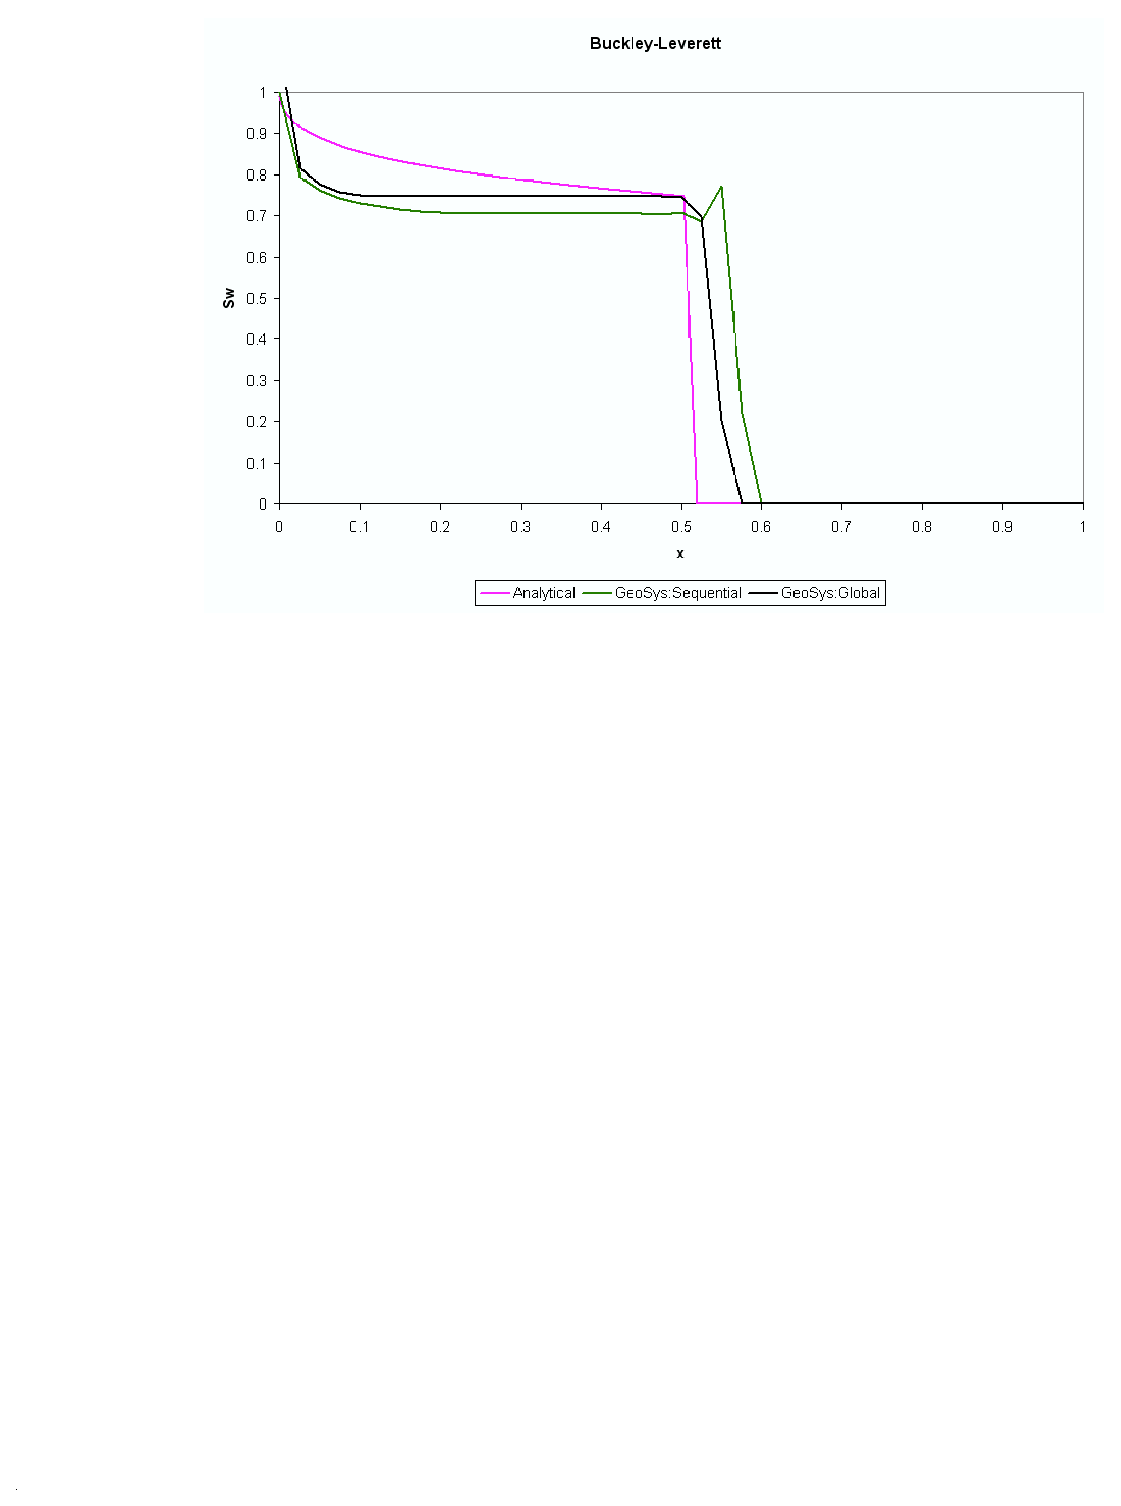
\includegraphics[scale=0.5]{HH/figures/PSGlobal.eps}
\end{center}
\vspace{-8.0cm}
\caption{}
\label{blg:comparison}
\end{figure}
\subsubsection*{\upshape\textbf{PS-Sequential}}
\hspace*{0.25cm}Adding (\ref{eq:w_eqn}) and (\ref{eq:nw_eqn}) with using the relation $S_{nw}+ S_w = 1$ and $p^{c}(S_w) = p_{nw} - p_w$, we get equation for wetting phase pressure, $p_{w}$ and non-wetting phase saturation, $S_{nw}$.
\begin{align}
 - n\frac{{\partial S_{nw}}}{{\partial t }} -
\nabla \cdot \left({\frac{{\mathbf k {k_{rel}}_w }}{{\mu_w }}\left( {\nabla p_w - \rho _w
\mathbf g} \right)} \right) = q_w
\label{eq:wfn_eqn}
\end{align}
\begin{align}
\nabla \cdot \left({\frac{{\mathbf k {k_{rel}}_w }}{{\mu_w }}\left( {\nabla p_w - \rho _w
\mathbf g} \right)} \right) +
\nabla \cdot \left({\frac{{\mathbf k {k_{rel}}_{nw} }}{{\mu_{nw} }}\left( {\nabla {p_w+p_c} - \rho _{nw}\mathbf g} \right)} \right) + \nonumber\\q_w + q_{nw} =0
\label{eq:nwfn_eqn}
\end{align}
In (\ref{eq:wfn_eqn}), non-wetting phase saturation, $S_{nw}$ can
be easily solved explicitly with the known pressure obtained from
(\ref{eq:nwfn_eqn}).

The analytical solution for the frontal location of the infiltrating fluid is derived and found there is the discrepancy with previous results (Helming and Huber $1998$, Figure $9$). In contrast to the previous results, the standard Galerkin-type method does tend to produce overestimated frontal infiltrating locations compared against the analytical solution. This can be explained by the diffusion term of the saturation originally omitted in the BL equation that makes purely advective transport. Handling this purely advective transport in general by the numerical models does introduces the numerical dispersion term naturally, and this added numerical dispersion can be interpreted by the saturation diffusion term.
\begin{figure}[!thb]
\begin{center}
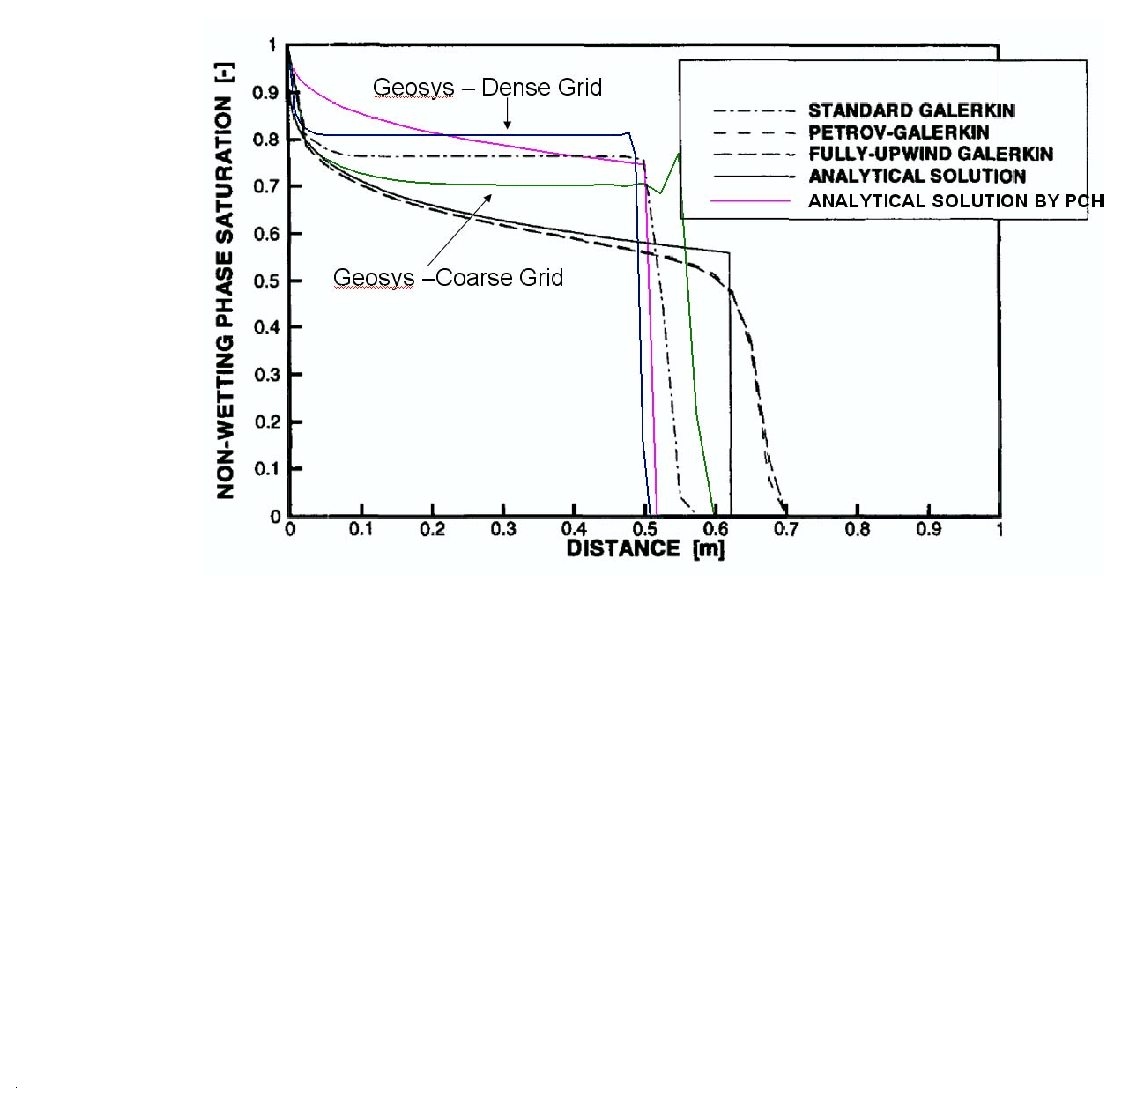
\includegraphics[scale=0.5]{HH/figures/PSSequential.eps}
\end{center}
\vspace{-5.0cm}
\caption{}
\label{bls:comparison}
\end{figure}
\subsubsection*{\upshape\textbf{Problem definition}}
\hspace*{0.25cm} Buckley and Leverett developed semi-analytical solution for the displacement of two immiscible fluid in porous media. Assume saturated $CO_2$ displacing $H_2O$ with constant fluid properties.
\subsubsection*{\upshape\textbf{Results}}
\hspace*{0.25cm} Here, we shown the saturation profile, $S_w$ in Fig. $18.1.7$ along $1~m$ column calculated with line element with space-time discretization of $\delta x = 0.025~m$ and $\delta t = 0.005~s$. The total simulation time is $0.4~s$; using the total-pressure-based pS-GLOBAL. Based on linear relation between saturation and relative permeability, saturation profile, $S_w$ is shown in Fig. $18.1.8$.\\\\
\begin{table}[!htb]
\begin{tabular}{lccr}
\hline\hline\noalign{\smallskip}
Property & Symbol & Value & Unit \\
\noalign{\smallskip}\hline\noalign{\smallskip}
Column length & $L$ & $m$ & $1.0$  \\
Porosity & $n$ & -- & $2.0\times10^{-1}$ \\
Permeability & $\kappa$ & $ m^2$ & $1.0\times 10^{-10}$ \\
Water dynamic viscosity &  $\mu_w$ & $Pa.s$ & $1.0\times10^{-3}$ \\
Gas dynamic viscosity & $\mu_{nw}$ & $Pa.s$ & $7.0343\times10^{-4}$ \\
Water density &  $\rho_w$ &$kg.m^{-3}$ & $1.0\times10^{3}$ \\
Gas density &  $\rho_{nw}$ & $kg.m^{-3}$ & $7.73\times10^{2}$ \\
Capillary pressure & $p^c(S)$ & $Pa$ & 0 \\
Relative permeability & $\kappa_{rel}(S)$ & -- & Brook-Corey functions \\
\noalign{\smallskip}\hline\hline
\end{tabular}
\caption{Material parameters for the BL problem.}
\end{table}
\begin{figure}[!thb]
\begin{center}
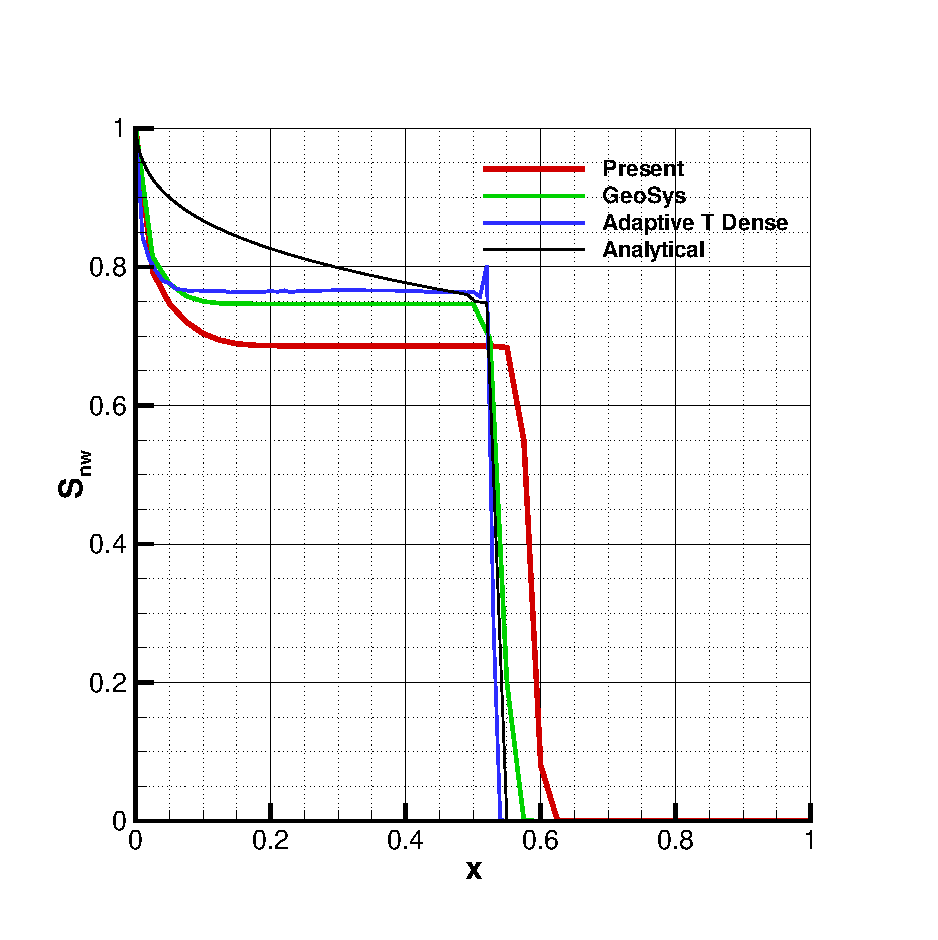
\includegraphics[scale=0.5]{HH/figures/BL-Sw.eps}
\end{center}
\caption{Saturation profile obtained with present analysis along with others.}
\label{bl:comparison}
\end{figure}
\begin{figure}[!thb]
\begin{center}
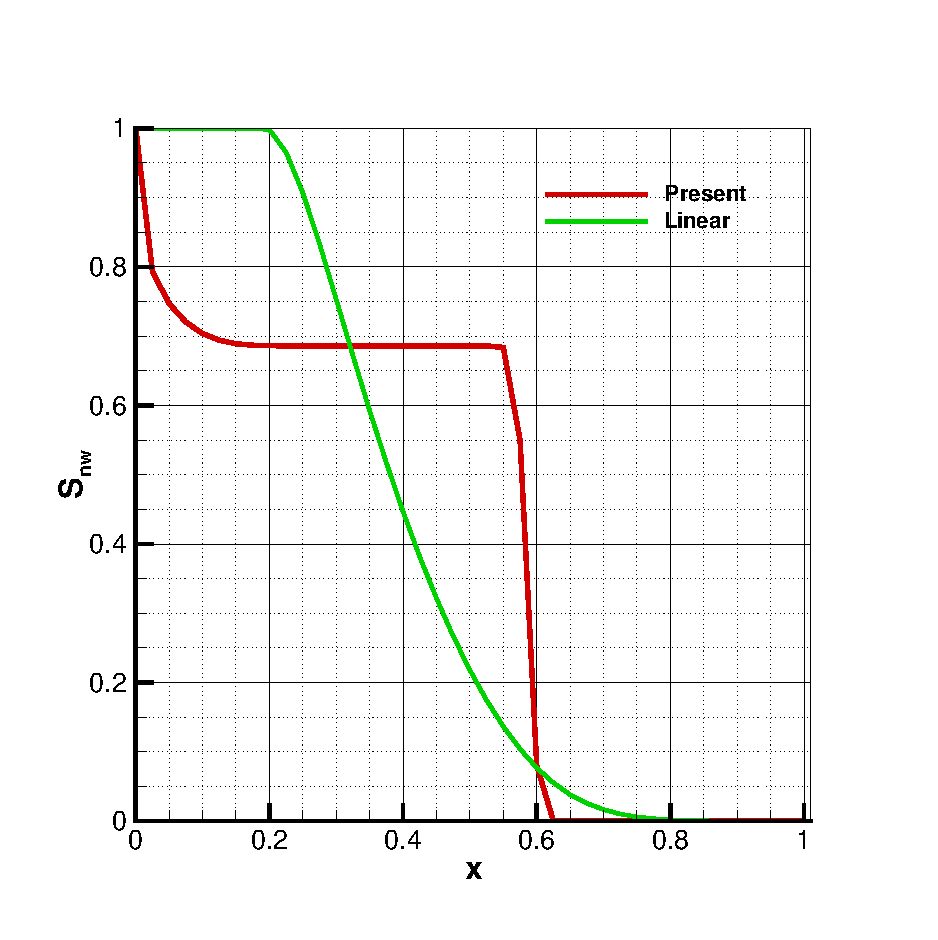
\includegraphics[scale=0.5]{HH/figures/BL-Sw-Linear.eps}
\end{center}
\caption{Saturation profile obtained with present analysis along with linear permeability and saturation relation.}
\label{bl:comparison}
\end{figure}
\clearpage
\subsubsection*{\upshape\textbf{Benchmark deposit}}
\begin{tabular}{|l|l|l|}
\hline
Benchmark & Problem type & Path in benchmark deposit \\
\hline
\emph{hm\_unsat}& HH & MULTIPHASE \\
\hline
\end{tabular}
\clearpage


%.........................................................................
%\subsection{McWorter problem}
%-------------------------------------------------------------------------
\subsection{\upshape\textbf{McWhorter problem}\label{MWPIsoTwoPhaseFlow}}
\subsubsection*{\upshape\textbf{Theory}}
It is assumed that the flow of both wetting and non-wetting phases can be adequately described by the Darcy's law if the phases are immiscible and incompressible.
\begin{equation}
n\frac{\partial S^{\gamma}}{\partial t} + \nabla \cdot \mathbf{q}^{\gamma} = 0, \gamma=w, nw
\label{eq:mcwtMassEq}
\end{equation}
\begin{equation}
\mathbf{q}^{\gamma}=-{\mathbf K} \lambda^{\gamma} \nabla p^{\gamma}
\label{eq:mcwtFluxEq}
\end{equation}
where $\lambda_w$ and  $\lambda_{nw}$ are mobility of wetting and non-wetting fluid. Both phase are linked by the state equation $S_w+S_{nw}=1$ and $p_c=p_g-p_w$. Here total flux, $\mathbf {q}_t=\mathbf {q}_w + \mathbf {q}_{nw}$ once $p_c$ is function of the $S_w$.


A formulation that is often used for two phase flow problem is so called fractional flow model. One of the attractive of this formulation is that the model become more accessible to analysis. Subtracting equation ($18.1.24$) for both phases we have.
\begin{equation}
\mathbf {q}_w=f \mathbf {q}_t- D \frac{\partial S_w}{\partial x}
\label{eq:McWhorterWetFlux}
\end{equation}
where 
\begin{equation*}
f=\frac{1}{1 + \frac{\lambda_{nw}}{\lambda_w}},~~~D=-\lambda_{nw} f \frac{\partial p_c}{\partial S_w}
\end{equation*}
First term on the right of equation (\ref{eq:McWhorterWetFlux}) is dicteted by rate at which flux is injected on the boundary and second term represent the addition impelling force due to gradient of capillary pressure. Put equation (\ref{eq:McWhorterWetFlux}) in equation ($18.1.23$) for wetting phase and assume that total flux, $\mathbf q_t$ is space invariant.
\begin{equation}
\frac{\partial }{\partial x}\left( D\frac{\partial S_w}{\partial x}\right) - \mathbf q_t \frac{\partial f}{\partial S_w}\frac{\partial S_w}{\partial x}=n \frac{\partial S_w}{\partial t}
\label{eq:McWhorterAnal}
\end{equation}
In the last benchmark (Buckley and Leveret) it is assume that force due to gradient of capillary pressure is very small as consequence of total flux, $\mathbf q_t$ is large hence suppressed the second order term in the equation.


Knowing  the capillarity effect, model verification need a comparison with an analytical solution based on one by McWhorter and Sunada ($1990$). They developed an exact quasi-analytical solution of equation (\ref{eq:McWhorterAnal}) for unidirectional displacement where non-wetting phase by wetting phase using the concept of a fractional flow function.


The fractional flow function is defined as ratio of wetting phase flux, $\mathbf q_w$ to the total flux, $\mathbf q_t$. It has shown that this ratio is function of $S_w$ only, when $\mathbf q_t$ is inversely related to square root of the time.
\newpage
\textbf{Problem definition}\\
The test benchmark problem for capillary effects is formulated as if the instantaneous displacement occurs in one-dimensional horizontal reservoir initially occupied by oil. Solution has been obtain through solving the governing equations ($18.1.12$) and ($18.1.13$) by pressure-pressure scheme described in sec (sec.\ref{sec:pp-scheme}). Different from the Buckley-Leverett problem, here flow is governed by capillary force when water saturation at the left end of the horizontal column is kept to be one, while the right end is kept to be no flux at all. So for no source term is accounted.
\vspace{-0.3cm}
\begin{figure}[H]
\begin{center}
\epsfig{figure=HH/figures/Schematic.eps,height=3cm}
\end{center}
\vspace{-0.6cm}
\caption{Schematic of the benchmark formulated to test McWhorter and Sunada's analytical solution.}
\label{mcwt:config}
\end{figure}
\vspace{-0.4cm}
\textbf{Results}\\
Based on the above discussion GeoSys produces agreeable solution. Fig. $18.1.10$ shows water saturation profile, $S_w$ with a fine grid along with $2.6m$ long horizontal column for different time steps. Line elements has been used with time and space discretization $\delta t=0.5s$ and $\delta x=0.05m$ respectively.
\begin{figure}[H]
\begin{center}
\epsfig{figure=HH/figures/pp_1d.eps,height=5cm}
\end{center}
\vspace{-0.4cm}
\caption{Water saturation, $S_w$ profile of the present result along with analytical solution based on one by McWhorter.}
\label{mcwt:ppModel}
\end{figure}
Here, we have solved exactly same problem using the total-pressure-based saturation model in sequential iterative coupling scheme.
\begin{figure}[H]
\begin{center}
\epsfig{figure=HH/figures/TPSMcWhorter.eps,height=5cm}
\end{center}
\caption{Water saturation, $S_w$ profile in sequential iterative coupling scheme.}
\label{mcwt:psModel}
\end{figure}
Unlike the pressure-pressure model, one downside for the total-pressure-based saturation model is less accurate for the problems dominated by capillarity (see Fig. $18.1.11$). Since the pressure-pressure model directly solves for capillary pressure as a primary variable, the model has an advantage for the capillary related problems. On the other hand, the total-pressure-based saturation model is limited to the problems when $d P_c/d S_w$ is close to zero. The condition for $d P_c/d S_w$ close to zero caused physically in the cases of fractures, shear zones and transitions between heterogeneities.
\begin{table}[!htb]
\begin{tabular}{lccr}
\hline\hline\noalign{\smallskip}
Property & Symbol & Value & Unit \\
\noalign{\smallskip}\hline\noalign{\smallskip}
Column length & $L$ & $m$ & $2.6$  \\
wetting dynamic viscosity &  $\mu_w$ & $Pa.s$ & $1.0\times10^{-3}$ \\
non-wetting dynamic viscosity & $\mu_{nw}$ & $Pa.s$ & $1.0\times10^{-3}$ \\
wetting phase density &  $\rho_w$ &$kg.m^{-3}$ & $1.0\times10^{3}$ \\
Non-wetting phase density &  $\rho_{nw}$ & $kg.m^{-3}$ & $1.0\times10^{3}$ \\
Permeability & $\mathbf K$ & $ m^2$ & $1.0\times 10^{-10}$ \\
Porosity & $n$ & $--$ & $3.0\times10^{-1}$ \\
Residual saturation of water &  $S_{rw}$ & $--$ & $0$ \\
Residual saturation of oil &  $S_{nrw}$ & $--$ & $0$ \\
Entry pressure &  $p_d$ & $Pa$ & $5.0\times10^{3}$ \\
Soil distribution index &  $\lambda$ & $--$ & $2.0$ \\
Capillary pressure & $p^c(S_{eff})$ & $Pa$ & Brooks-Corey model\\
Relative permeability & $\kappa_{rel}(S_{eff})$ & $--$ & Brooks-Corey model \\
\noalign{\smallskip}\hline\hline
\end{tabular}
\caption{Material parameters for the McWhorter problem.}
\end{table}
\clearpage
\subsubsection*{\upshape\textbf{Benchmark deposit}}
\begin{tabular}{|l|l|l|}
\hline
Benchmark & Problem type & Path in benchmark deposit \\
\hline
\emph{mcwt}& H2 & McWhorter \\
\hline
\end{tabular}
\clearpage


%.........................................................................
%\subsection{McWorter problem}
%-------------------------------------------------------------------------
\subsection{\upshape\textbf{Kueper problem}}
\subsubsection*{\upshape\textbf{Theory}}
The former two benchmarks (Buckley-Leverett and McWorter)used for verification, both schemes are further tested for model validation with the benchmark chosen to test two-phase flow in heterogeneous media. Kueper and Frind (1991) developed the model to simulate their experiment for DNAPL penetration (Kueper et al., $1989$). The simultaneous movement of a dense non-wetting phase (DNAPL) through an initially wetting phase (water) saturated heterogeneous porous media may be represented mathematically as a case of two-phase flow. A distinctive feature of the solution is that the primary variables solved for, wetting phase pressure and wetting phase saturation, are both existent throughout the solution domain regardless of whether the non-wetting phase is present.


The continuity equation of each phase ($\gamma$) can be defined by
\begin{equation}
\frac{\partial (n {\rho}^{\gamma} S^{\gamma})}{\partial t} + \nabla \cdot ({\rho}^{\gamma} \mathbf{q}^{\gamma}) = \mathbf{Q}^{\gamma}, \gamma=w, nw
\label{eq:mcwtMassEq}
\end{equation}
where $n$ is porosity, $S^{\gamma}$ is saturation, $\rho^{\gamma}$ is density, $\mathbf{Q}^{\gamma}$ is a source or sink term, and $\mathbf{q}^{\gamma}$ is the Darcy velocity for phase $\gamma$ defined by
\begin{equation}
\mathbf{q}^{\gamma}=-{\mathbf K} \frac{\kappa_r^{\gamma}}{\mu^{\gamma}}(\nabla p^{\gamma}-{\rho}^{\gamma} \mathbf{g}), \gamma=w, nw
\label{eq:mcwtFluxEq}
\end{equation}

where $\kappa_r^{\gamma}$ is relative permeability, $\mu^{\gamma}$ is viscosity, $p^{\gamma}$ is pressure for phase $\gamma$, $\textbf{K}$ is intrinsic permeability tensor and $\mathbf{g}$ is the gravitational vector.  


Inherently for saturation, the sum of all saturation in pore space is
\begin{equation}
{\sum S^{\gamma}}=1
\label{eq:mcwtFluxEq}
\end{equation}
Assuming relative preference (i.e., wettability) of the fluid to media exists and it is not negligible, the capillary pressures relation for a two-phase system is defined over representative elementary volume (REV) by 
\begin{equation}
p_c=p_{nw}-p_w
\label{eq:mcwtFluxEq}
\end{equation}                                                 
where $p_c$ is capillary pressure, $p_{nw}$ is pressure for the non-wetting phase fluid and $p_w$ is the wetting phase fluid. 


\textbf{Problem definition}\\\
A $60cm\times80cm\times0.6cm$ parallel-plate glass-lined cell was packed with four types of sands and initially fully saturated with water. The configuration of the assembled sand lenses and the two sets of the boundary conditions for the $p_w-S_{nw}$ and $p_c-p_{nw}$ schemes are illustrated in Figure $18.1.12$. Concerning to the constitutive relation between relative permeability and saturation and capillary pressure and saturation, they have used the Brooks-Corey model. 


Properties of Sands for the Brooks-Corey model are measured experimentally and summarized in table. The numerical solutions obtained from the $p_w-S_{nw}$ scheme and the $p_c-p_{nw}$ scheme for the benchmark Kueper and Frind ($1991$) are compared against each other in Figure $18.1.13$. 
\begin{figure}[H]
\begin{center}
\epsfig{figure=HH/figures/KueperConfiguration.eps,height=5cm}
\end{center}
\caption{Configuration of heterogeneous media in parallel-plate cell.}
\label{mcwt:psModel}
\end{figure}

\subsubsection*{\upshape\textbf{Fluid and medium properties with numerical space and time discretization.}}
\begin{tabular}{|l|l|l|l|}
\hline
Fluid properties & Unit & Wetting fluid	& Non-wetting fluid \\
\hline
Density &	$kg.m^{-3}$ &	$1.0\times10^3$ &	$1.0\times10^3$ \\ 
\hline
Viscosity &	$Pa\cdots$ & $1.0\times10^{-3}$ &	$1.0\times10^{-3}$ \\
\hline
Residual saturation &	- &	0.0 &	0.0 \\
\hline
Maximum saturation &	- &	1.0 &	1.0 \\
\hline
\end{tabular}

\begin{tabular}{|l|l|l|}
\hline
Medium properties & Unit & Medium\\
\hline
$\Delta x$ & m &	0.01 \\
\hline
$\Delta t$ & s &	100 \\
\hline
Porosity & - &	0.3 \\
\hline
Intrinsic permeability & $m^2$ & $1\times10^{-10}$ \\
\hline
Brook-Corey's index &	- &	2 \\
\hline
Entry pressure & Pa & $5\times10^3$ \\
\hline
\end{tabular}

\subsubsection*{\upshape\textbf{Hydraulic properties of sands for the Brooks-Corey model.}}
\begin{tabular}{|l|l|l|l|l|l|}
\hline
Property & $P_d$(Pa) & $\lambda$(-) &	$S_{wr}$(-) &	k($m^2$) &	$n$(-) \\
\hline
1	& 369.73 & 3.86	& 0.078	& $5.04\times10^{-10}$ & 0.40 \\ 
\hline
2	& 434.45 & 3.51 & 0.069 &	$2.05\times10^{-10}$ & 0.39 \\
\hline
3	& 1323.95 &	2.49 & 0.098 &	$5.26\times10^{-11}$ & 0.39 \\
\hline
4	& 3246.15	& 3.30 & 0.189 & $8.19\times10^{-12}$ &	0.41 \\
\hline
\end{tabular}


\begin{figure}[H]
\begin{center}
\epsfig{figure=HH/figures/Kueper.eps,height=12cm}
\end{center}
\caption{Comparison of the results obtained from the $p_w-S_{nw}$ and $p_c-p_{nw}$ schemes. The second column shows good agreement with observed distribution of DNAPL of the experiment (Kueper and Frind $1991$).}
\label{mcwt:psModel}
\end{figure}
Both schemes produce DNAPL plume propagation physically until the plume reaches to the less previous media under the top medium in the model domain. The striking difference occurs at the interface between these two media. While the pwSnw scheme simulates the plume to infiltrate into the less previous medium, the $p_c-p_{nw}$ scheme does the plume to bypass the less previous medium. A similar experiment and simulation comparison against experimental observation are also conducted by Helming and Huber ($1998$). They have reported unphysical fluid behavior captured by the $p_w-S_{nw}$ scheme, and this phenomenon can be avoided with fully upwind technique (Helming and Huber, $1998$). 
\subsubsection*{\upshape\textbf{Benchmark deposit}}
\begin{tabular}{|l|l|l|}
\hline
Benchmark & Problem type & Path in benchmark deposit \\
\hline
\emph{Kueper}& H2 & MULTIPHASE \\
\hline
\end{tabular}

%\subsection{Heat Pipe problem}
%-------------------------------------------------------------------------
\subsection{\upshape\textbf{Heat Pipe problem}\label{HPPNonIsoTwoPhaseFlow}}
\subsubsection*{\upshape\textbf{Theory}}
When an unsaturated porous medium subjected to a constant heat flux and the temperature is sufficiently high, water is heated and vaporizes. Vapor flows under its pressure gradient towards cooler end where it condenses. Vaporization and condensation produce a liquid saturation gradient, creating a capillary pressure gradient inside the porous medium. Condensate flows towards the hot end under the influence of a capillary pressure gradient. This is a heat pipe in an unsaturated porous medium


Udell and Fitch derived the pressure gradient of the each phases in two-phase flow with heat transfer. The generalized form of the Darcy's law is used to calculate velocity fields. 
\begin{equation}
\frac{d p^g}{d x} = \frac{\eta q \nu^g}{\mathbf k k_{\mathrm {rg}} H_{\mathrm {vap}}}
\label{eq:HP1}
\end{equation}
\begin{equation}
\frac{d p^l}{d x} =- \frac{\eta q \nu^l}{\mathbf k k_{\mathrm {rl}} H_{\mathrm {vap}}}
\label{eq:HP2}
\end{equation}
where, $\eta$ is the ratio of heat transport caused by convection to the total heat-flux $q$ (see Helming [1997]). $p$ is phase pressure; $\nu^\gamma=\frac{\mu\gamma}{\rho^\gamma}$; $x$ is space coordinate in the x-direction; $\mathbf k$ is intrinsic permeability; $k_{r\gamma}$ is relative permeability and $H_{\mathrm {vap}}$ is latent heat of water. $\gamma$ is the phase superscript and $g, l$ stand for gas and liquid phase, respectively. Gas pressure is the sum of two partial pressure, i.e. $p^g=p^g_a+p^g_w$.

The density of gas phase is sum of air and vapor density. Air density is according to ideal gas equation, i.e.
\begin{equation}
\rho_{\mathrm {ga}}=\frac{M_a p_a}{RT} 
\label{eq:HP3}
\end{equation}
The energy transport is described by Zhou et al. [1990] as
\begin{equation}
q=-\kappa_{\mathrm {app}}\frac{\partial d T}{d x} + \dot m_{\mathrm {vap}} H_{\mathrm {vap}}
\label{eq:HP4}
\end{equation}
where, $T$ is temperature, $\kappa_{\mathrm {app}}$ is apparent thermal conductivity.

Since capillary pressure is the difference of phase pressure, hence from Eq. 1, the capillary pressure gradient is
\begin{equation}
\frac{d p^c}{d x} = \frac{\eta q}{\mathbf k H_{\mathrm {vap}}}\left[\frac{\nu^g}{k_{\mathrm {rg}}} + \frac{\nu^l}{k_{\mathrm {rl}}}\right]
\label{eq:HP5}
\end{equation}
Brooks-Corey has presented water saturation -capillary pressure relation in the following form
\begin{equation}
S=\left(\frac{Pd}{p^c}\right)^\lambda
\label{eq:HP6}
\end{equation}
By comparing this with Leverett's [1941] non-dimensional form we get $Pd=\sigma_0\left(\frac{n}{\mathbf k}\right)^{0.5}$ and $n$ is medium porosity. $\sigma_0$ is interfacial tension at reference temperature $T_0$. Here, $S$ is scaled as following 
\begin{equation}
S=\frac{S_{\mathrm {w}}-S_{\mathrm {lr}}}{1-S_{\mathrm {lr}}-S_{\mathrm {gr}}}
\label{eq:HP7}
\end{equation}
The constant $S_{\mathrm {lr}}; S_{\mathrm {gr}}$ are residual saturations. And for interfacial tension we have used following correlation given by Olivella and Gens[2000].
\begin{equation}
\sigma( T)={0.3258C^{1.256}} - {0.148C^{2.256}};~~ T\le 633.15 \mathrm K
\label{eq:surface_tension}
\end{equation}
where, $C=1.0-\frac{T}{647.3~K}$\\

Brooks-Corey relative permeabilities relation are 
\begin{equation}
\mathbf k_{\mathrm {rg}}=\left(1-S\right)^2 \left(1-S^{\frac{2+\lambda}{\lambda}}\right);~~~\mathbf k_{rl}=S^{\frac{2+3\lambda}{\lambda}}
\label{eq:HP8}
\end{equation}
Using Eqs. (\ref{eq:HP5}-\ref{eq:HP6}), we can write following forms of saturation gradient.
\begin{equation}
\frac{d S}{d x}=\frac{S^{1.5}}{P_d}\frac{2\eta q}{\mathbf k H_{\mathrm {vap}}}\left[\frac{\nu^g}{k_{\mathrm {rg}}} + \frac{\nu^l}{k_{\mathrm {rl}}}\right]
\label{eq:HP9}
\end{equation}
Now Eq. (\ref{eq:HP9}) is integrated over two-phase zone. Where two-phase zone can be defined by imposing the limits of integration (see Udell [1985]): $S=S_0$ at $x=0$ and $S=S_1$ at $x=L$.

The saturation vapor density $\rho_{\mathrm {sat}}$, is depending on temperature, and estimated by following relation
\begin{equation}
\rho_{\mathrm {sat}}=1.0\times10^{-3}\exp\left(a-\frac{b}{T}\right)
\label{eq:HP10}
\end{equation}
where, constants $a=19.81$ and $b=4975.9$.

In the porous medium, we must account for a decrease in vapor density due to capillarity. The amount of decrease in vapor density is describe by Kelvin equation as follow
\begin{equation}
\rho_{\mathrm {gw}}=\rho_{\mathrm {sat}}\exp\left(-\frac{M_{\mathrm w} p^c}{\rho^l RT}\right)
\label{eq:HP11}
\end{equation}
where $M_{\mathrm w}$ is water molecular weight; $\rho^l$ is liquid density and $R$ is universal gas constant. From Eqs. (\ref{eq:HP10}-\ref{eq:HP11}), we get temperature as function of vapor density and capillary pressure as
\begin{equation}
T=\frac{A}{B}
\label{eq:HP12}
\end{equation}
where
\begin{equation*}
 A=b+\frac{M_{\mathrm w} p^c}{\rho^l R}; B=a-3 -\log\left(\rho_{\mathrm {gw}}\right)
 \label{eq:HP20}
\end{equation*}


$\rho_{\mathrm {gw}}$ is changing with temperature which makes difficulty for temperature calculation. Hence we need to know temperature gradient which is possible by Eq. (\ref{eq:HP12}) along with vapor pressure gradient 
\begin{equation}
\frac{d p_{\mathrm{gw}}}{d x} = \frac{\eta q \nu^g_w}{\mathbf k k_{\mathrm {rg}} H_{\mathrm {vap}}}
\label{eq:HP18}
\end{equation}
Form of the temperature gradient
\begin{equation}
\frac{d T}{d x}=\frac{\frac{B M_{\mathrm w}}{\rho^l R} \frac{d p^c}{d x} + \frac{A}{p_{\mathrm{gw}}} \frac{d p_{\mathrm{gw}}}{d x}}{B^2+\frac{A}{T}}
\label{eq:HP13}
\end{equation}
Apparent thermal conductivity can be get from heat flux divided by temperature gradient (see Udell [1985].


The coupled differential Eqs. (\ref{eq:HP1}), (\ref{eq:HP5}), (\ref{eq:HP9}) and (\ref{eq:HP13} ) are integrated by using Euler method with following boundary condition at $x=0$:
\begin{equation}
S=S_0;~~~ p^g=p^g_0;~~~p^c=p^c_0;~~~T=T_0
\label{eq:HP14}
\end{equation}
Material parameters are presented in Table \ref{tab:HP1}.\\

\textbf{Problem definition}\\\\
The test benchmark problem for heat pipe effects is formulated in one-dimensional. 
Horizontal column of length $2.6$~m is filled with fluid subjected to a constant heat flux at the right end where left end temperature maintained below to the saturation temperature.
\begin{figure}[htb]
\begin{center}
\epsfig{figure=HH/figures/Geo.eps,height=1.25cm}
\end{center}
\caption{Schematic of the benchmark.}
\label{Fig:HP1}
\end{figure}\\


\textbf{Results}\\\\
In order to establish the non-isothermal two-phase flow in the OpenGeoSys, we have verified numerical solutions with analytical results. Profile of water saturation $S_{\mathrm w}$, gas phase pressure $p^g$, liquid phase pressure $p^l$ and temperature $T$ are presented in Figs. \ref{Fig:HP2}, and \ref{Fig:HP4}. Found that numerical solutions are agreeable. Line elements has been used with variable time steps and a non uniform space discretization.
\begin{figure}[thbp]
\centerline{
\psfig{figure=HH/figures/S-Pc.eps,height=3.0in,width=3.0in}
\psfig{figure=HH/figures/Pw-Pg.eps,height=3.0in,width=3.0in}}
\caption{Comparison of water saturation and pressure profiles from present solution with analytical solution.}
\label{Fig:HP2}
\end{figure}
A finite element approach has been developed for the nonisothermal two-phase flow model based on the $ppT$ formulation. We used a combined monolithic/ staggered coupling scheme i.e. monolithic for the two-phase flow and staggered for the heat transport.
\begin{figure}[htb]
\begin{center}
\epsfig{figure=HH/figures/Tg.eps,height=8cm}
\end{center}
\caption{Comparison of temperature profile from present solution with analytical solution.}
\label{Fig:HP4}
\end{figure}
\begin{table}[htbp]
\caption{Material parameters for the heat pipe problem.}
\label{tab:HP1}
\begin{tabular}{l*{4}{l}r}
\hline
\textbf{Meaning} & \textbf{Symbol} &  \textbf{Value} &  \textbf{Unit} \\
\hline
Column length & $L$ & $\mathrm m$ & $2.6$  \\
Liquid dynamic viscosity &  $\mu^l$ & $\mathrm {Pa.s}$ & $1.0\times10^{-3}$ \\
Gas dynamic viscosity & $\mu^g$ & $\mathrm {Pa.s}$ & $1.0\times10^{-5}$ \\
Liquid density &  $\rho^l$ &$\mathrm {kg.m^{-3}}$ & $1.0\times10^{3}$ \\
Permeability & $\mathbf k$ & $ \mathrm {m^2}$ & $1.0\times 10^{-13}$ \\
Porosity & $n$ & $--$ & $0.3$ \\
Residual saturation of water &  $S_{\mathrm{rl}}$ & $--$ & $0.2$ \\
Residual saturation of oil &  $S_{\mathrm{rg}}$ & $--$ & $0$ \\
Soil distribution index &  $\lambda$ & $--$ & $2.0$ \\
Capillary pressure & $p^c(S)$ & $\mathrm {Pa}$ & Brooks-Corey model\\
Relative permeability & $\kappa_{\mathrm {r\gamma}}(S)$ & $--$ & Brooks-Corey model \\ \hline
\end{tabular}
\end{table}

\clearpage
\subsubsection*{\upshape\textbf{Benchmark deposit}}
\begin{tabular}{|l|l|l|}
\hline
Benchmark & Problem type & Path in benchmark deposit \\
\hline
\emph{HeatPipe}& H2 & MULTIPHASE \\
\hline
\end{tabular}
\clearpage
